\documentclass[11pt,a4paper]{article}
\usepackage[margin=1in]{geometry}
\usepackage{amsmath,amssymb,amsthm}
\usepackage{hyperref}
\usepackage{enumitem}
\usepackage{graphicx}
\usepackage{algorithm}
\usepackage{algpseudocode}
\usepackage{tikz}
\usetikzlibrary{arrows.meta,positioning,calc}

\theoremstyle{definition}
\newtheorem{definition}{Definition}
\newtheorem{construction}{Construction}
\newtheorem{property}{Property}

\title{Shielded Payments for Tangle Blueprints:\\
Anonymous Pay-Per-Use Cloud Services via\\Cross-Chain Shielded Pools and Prepaid Credits}

\author{
  Drew Stone\\
  \texttt{drew@tangle.tools}\\
  Tangle Network
}

\date{March 2026}

\begin{document}
\maketitle

\begin{abstract}
We present a privacy-preserving payment system for Tangle's Blueprint service protocol that enables anonymous pay-per-use access to cloud services including LLM inference, compute, and storage. The system composes three layers: (1) a cross-chain variable-amount shielded pool based on the Webb Anchor System~\cite{webb} supporting multi-asset wrapping, (2) a gateway contract that bridges anonymous pool withdrawals to Tangle's service lifecycle, and (3) a prepaid credit scheme where a single on-chain zero-knowledge proof funds an account from which many jobs are authorized via cheap EIP-712 signatures. The construction requires no modifications to Tangle's audited core contracts and introduces only 664 lines of new Solidity as auditable surface. We provide formal definitions, security properties, and a complete implementation with 30 passing tests including end-to-end flows.
\end{abstract}

\section{Introduction}

Decentralized service marketplaces face a fundamental tension: users want privacy when consuming services, but operators need payment guarantees before performing work. Existing systems force users to reveal their identity with every payment, creating surveillance vectors that centralized alternatives avoid through corporate privacy policies rather than cryptographic guarantees.

Buterin and Crapis~\cite{zkapi} proposed ``ZK API Usage Credits'' for anonymous LLM inference: users deposit into a smart contract and generate zero-knowledge proofs to authorize each API call without revealing their identity. While elegant, generating a zkSNARK proof per API call is impractical---proof generation takes $\sim$10 seconds and costs $\sim$300k gas on-chain.

We extend this idea with a two-phase design:
\begin{enumerate}[nosep]
  \item \textbf{Funding phase}: One zkSNARK proof (VAnchor withdrawal) creates a pseudonymous credit account.
  \item \textbf{Spending phase}: Many ECDSA signatures ($\sim$3k gas each) authorize individual job payments.
\end{enumerate}

This paper describes the complete system built on Tangle's existing Blueprint protocol, reusing the audited Webb Protocol shielded pool~\cite{webb} for the funding phase and introducing a minimal credit contract for the spending phase.

\subsection{Contributions}

\begin{itemize}[nosep]
  \item A gateway architecture that bridges VAnchor shielded pools to Tangle's service lifecycle with zero modifications to the core protocol.
  \item A prepaid credit scheme using EIP-712 typed signatures that amortizes the cost of a single ZK proof over arbitrarily many service invocations.
  \item Multi-asset wrapping via \texttt{FungibleTokenWrapper}, allowing users to deposit any supported stablecoin into a single anonymity pool.
  \item An implementation with 664 lines of new Solidity, 30 passing Forge tests, and a TypeScript SDK.
\end{itemize}

\section{Preliminaries}

We adopt the notation from the Webb Protocol~\cite{webb}. Let $H : \mathbb{F}_p^* \to \mathbb{F}_p$ denote a collision-resistant hash function (Poseidon). Let $(\mathsf{pk}, \mathsf{sk})$ denote a keypair where $\mathsf{pk} = H(\mathsf{sk})$.

\begin{definition}[UTXO Commitment]
A commitment to a UTXO with chain identifier $i$, value $v$, public key $\mathsf{pk}$, and blinding factor $r \xleftarrow{\$} \mathbb{F}_p$ is:
$$\mathsf{cm} = H(i, v, \mathsf{pk}, r)$$
\end{definition}

\begin{definition}[Nullifier]
The nullifier for a commitment $\mathsf{cm}$ at Merkle path index $j$ with signature $\sigma = H(\mathsf{sk}, j, \mathsf{cm})$ is:
$$\mathsf{sn} = H(\mathsf{cm}, j, \sigma)$$
\end{definition}

\begin{definition}[Cross-Chain Merkle Membership]
Given a set of Merkle roots $\mathbf{MR} = \{\mathsf{MR}_1, \ldots, \mathsf{MR}_k\}$ from $k$ connected anchor instances, a commitment $\mathsf{cm}$ satisfies cross-chain membership if:
$$\mathsf{MR}_{\mathsf{cm}} := \mathsf{reconstruct}(\mathsf{cm}, \mathsf{path}(\mathsf{cm}), H) \in \mathbf{MR}$$
\end{definition}

\begin{definition}[Tangle Service]
A \emph{service} is a running instance of a \emph{blueprint} (service template) with assigned operators. Services support three pricing models: \textsc{PayOnce} (upfront), \textsc{Subscription} (periodic escrow), and \textsc{EventDriven} (per-job). Users interact via \emph{permitted callers} authorized at service creation.
\end{definition}

\section{System Architecture}

The system comprises three contracts and one SDK:

\begin{center}
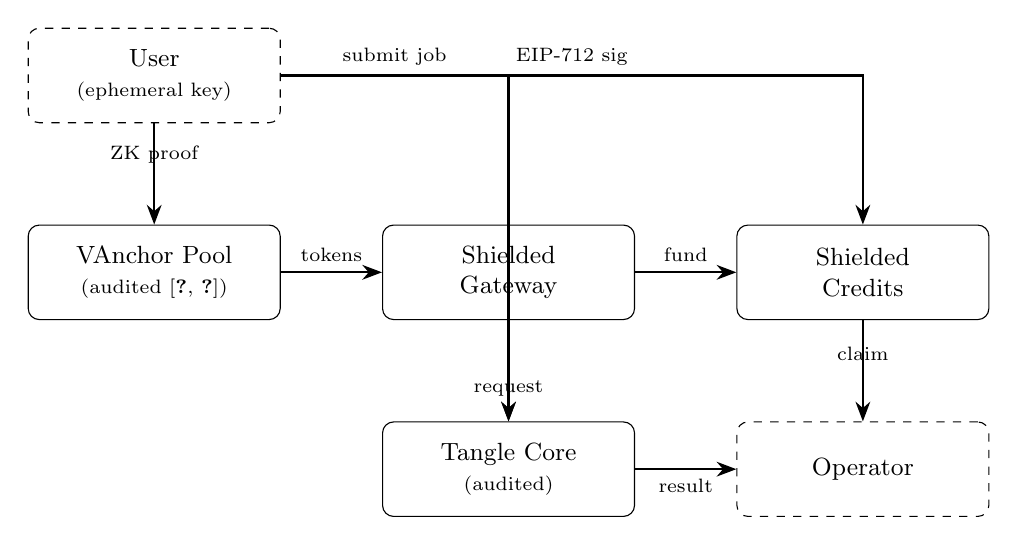
\begin{tikzpicture}[
  box/.style={draw, rounded corners, minimum width=3.2cm, minimum height=1.2cm, align=center, font=\small},
  arr/.style={-{Stealth[length=2.5mm]}, thick},
  lbl/.style={font=\scriptsize, midway, above}
]
  \node[box] (pool) at (0,0) {VAnchor Pool\\{\scriptsize (audited~\cite{webb,veridise})}};
  \node[box] (gw) at (4.5,0) {Shielded\\Gateway};
  \node[box] (credits) at (9,0) {Shielded\\Credits};
  \node[box] (tangle) at (4.5,-2.5) {Tangle Core\\{\scriptsize (audited)}};
  \node[box, dashed] (user) at (0,2.5) {User\\{\scriptsize (ephemeral key)}};
  \node[box, dashed] (op) at (9,-2.5) {Operator};

  \draw[arr] (user) -- node[lbl] {ZK proof} (pool);
  \draw[arr] (pool) -- node[lbl] {tokens} (gw);
  \draw[arr] (gw) -- node[lbl] {fund} (credits);
  \draw[arr] (gw) -- node[lbl, below] {request} (tangle);
  \draw[arr] (user) -| node[lbl, near start] {EIP-712 sig} (credits);
  \draw[arr] (user) -- ++(4.5,0) node[lbl] {submit job} -- (tangle);
  \draw[arr] (credits) -- node[lbl] {claim} (op);
  \draw[arr] (tangle) -- node[lbl, below] {result} (op);
\end{tikzpicture}
\end{center}

\subsection{VAnchor Shielded Pool (Existing, Audited)}

We reuse the Variable Asset Anchor System from the Webb Protocol~\cite{webb} without modification. The VAnchor implements a UTXO-based shielded pool with:

\begin{itemize}[nosep]
  \item \textbf{Variable amounts}: Unlike fixed-denomination mixers, UTXOs carry arbitrary values.
  \item \textbf{JoinSplit transactions}: 2-in-2-out or 16-in-2-out for splits, merges, and transfers.
  \item \textbf{Cross-chain roots}: \texttt{ManyMerkleProof} validates a commitment against roots from any connected chain.
  \item \textbf{Multi-asset wrapping}: \texttt{FungibleTokenWrapper} accepts multiple ERC20s (e.g., USDC, USDT, DAI) into a single wrapped token, maximizing the anonymity set.
\end{itemize}

The zkSNARK relation for VAnchor transactions (from~\cite{webb}, Example 2):

\begin{construction}[VAnchor Transaction Gadget]
For public inputs $x = \{\mathsf{public\_amount}, \mathbf{MR}, i, \{\mathsf{sn}_k\}_{k \leq \mathsf{INS}}, \{\mathsf{cm}_o\}_{o \leq \mathsf{OUTS}}\}$ and private witness $\mathbf{w} = \{v_k, r_k, \mathsf{sk}_k, j_k, \mathsf{path}(\mathsf{cm}_k)\}_{k \leq \mathsf{INS}} \cup \{v_o, r_o, i_o, \mathsf{sk}_o, j_o\}_{o \leq \mathsf{OUTS}}$, the relation $\mathcal{R}$ enforces:

\begin{align}
  &\{\mathsf{pk}_k := H(\mathsf{sk}_k)\}_{k \leq \mathsf{INS}} \\
  &\{\mathsf{cm}_k := H(i, v_k, \mathsf{pk}_k, r_k)\}_{k \leq \mathsf{INS}} \\
  &\{\sigma_k := H(\mathsf{sk}_k, j_k, \mathsf{cm}_k)\}_{k \leq \mathsf{INS}} \\
  &\{\mathsf{MR}_{\mathsf{cm}_k} := \mathsf{reconstruct}(\mathsf{cm}_k, \mathsf{path}(\mathsf{cm}_k), H) \in \mathbf{MR}\}_{k \leq \mathsf{INS}} \\
  &\mathsf{public\_amount} + \sum_{k \leq \mathsf{INS}} v_k = \sum_{o \leq \mathsf{OUTS}} v_o \\
  &\{\mathsf{sn}_k\}_{k \leq \mathsf{INS}} \text{ are distinct}
\end{align}
\end{construction}

\subsection{Shielded Gateway}

The \texttt{ShieldedGateway} contract is a stateless proxy between the VAnchor and Tangle. It executes a VAnchor withdrawal (which validates the zkSNARK proof and marks nullifiers as spent), receives the withdrawn tokens, and atomically forwards them to one of three Tangle operations:

\begin{enumerate}[nosep]
  \item \texttt{shieldedRequestService}: Creates a new service with the gateway as owner and user-specified ephemeral addresses as permitted callers.
  \item \texttt{shieldedFundService}: Tops up an existing service's escrow.
  \item \texttt{shieldedFundCredits}: Funds a prepaid credit account (Section~\ref{sec:credits}).
\end{enumerate}

\begin{property}[Atomicity]
The gateway never holds funds beyond a single transaction. Every token received from the VAnchor is forwarded in the same call. If the forward fails, the entire transaction reverts (including the VAnchor withdrawal).
\end{property}

\begin{property}[Non-Linkability]
The gateway stores no mapping between VAnchor nullifiers and Tangle service/credit identifiers. An observer sees \texttt{VAnchor} $\to$ \texttt{Gateway} $\to$ \texttt{Tangle/Credits} but cannot determine which pool depositor initiated the operation.
\end{property}

\subsection{Shielded Credits}\label{sec:credits}

The core contribution: a prepaid credit system that amortizes a single ZK proof over many service invocations.

\begin{definition}[Credit Account]
A credit account is identified by a commitment $\mathsf{C} = \mathsf{keccak256}(\mathsf{pk}_s \| \mathsf{salt})$ where $\mathsf{pk}_s$ is an ephemeral ECDSA public key and $\mathsf{salt} \xleftarrow{\$} \{0,1\}^{256}$. The account state is:
$$\mathsf{Account}[\mathsf{C}] = (\mathsf{pk}_s, \mathsf{token}, \mathsf{balance}, \mathsf{nonce})$$
\end{definition}

\begin{definition}[Spend Authorization]
A spend authorization for credit account $\mathsf{C}$ is an EIP-712 typed data signature:
$$\mathsf{SpendAuth} = \mathsf{Sign}_{\mathsf{sk}_s}\Big(\mathsf{C}, \mathsf{serviceId}, \mathsf{jobIndex}, \mathsf{amount}, \mathsf{operator}, \mathsf{nonce}, \mathsf{expiry}\Big)$$
where $\mathsf{sk}_s$ is the ephemeral private key corresponding to $\mathsf{pk}_s$.
\end{definition}

\subsubsection{Credit Protocol}

\begin{algorithm}[H]
\caption{Credit Lifecycle}
\begin{algorithmic}[1]
\Procedure{FundCredits}{$\mathsf{token}, \mathsf{amount}, \mathsf{C}, \mathsf{pk}_s$}
  \State Pull $\mathsf{amount}$ of $\mathsf{token}$ from caller (Gateway)
  \If{$\mathsf{Account}[\mathsf{C}]$ exists}
    \State \textbf{require} $\mathsf{Account}[\mathsf{C}].\mathsf{pk}_s = \mathsf{pk}_s$ \Comment{Immutable key}
  \Else
    \State $\mathsf{Account}[\mathsf{C}] \gets (\mathsf{pk}_s, \mathsf{token}, 0, 0)$
  \EndIf
  \State $\mathsf{Account}[\mathsf{C}].\mathsf{balance} \mathrel{+}= \mathsf{amount}$
\EndProcedure

\Statex

\Procedure{AuthorizeSpend}{$\mathsf{auth}$}
  \State $\mathsf{acct} \gets \mathsf{Account}[\mathsf{auth.C}]$
  \State \textbf{require} $\mathsf{auth.nonce} = \mathsf{acct.nonce}$ \Comment{Strict ordering}
  \State \textbf{require} $\mathsf{auth.amount} \leq \mathsf{acct.balance}$
  \State \textbf{require} $\mathsf{block.timestamp} \leq \mathsf{auth.expiry}$
  \State \textbf{require} $\mathsf{ecrecover}(\mathsf{digest}(\mathsf{auth})) = \mathsf{acct.pk}_s$
  \State $\mathsf{acct.balance} \mathrel{-}= \mathsf{auth.amount}$; \; $\mathsf{acct.nonce}\mathrel{+}{+}$
  \State $\mathsf{authHash} \gets H(\mathsf{auth.C}, \mathsf{auth.serviceId}, \mathsf{auth.jobIndex}, \mathsf{auth.nonce})$
  \State Store $\mathsf{Pending}[\mathsf{authHash}] \gets (\mathsf{auth.amount}, \mathsf{auth.operator})$
  \State \Return $\mathsf{authHash}$
\EndProcedure

\Statex

\Procedure{ClaimPayment}{$\mathsf{authHash}, \mathsf{recipient}$}
  \State \textbf{require} $\mathsf{msg.sender} = \mathsf{Pending}[\mathsf{authHash}].\mathsf{operator}$
  \State \textbf{require} not $\mathsf{Claimed}[\mathsf{authHash}]$
  \State $\mathsf{Claimed}[\mathsf{authHash}] \gets \mathsf{true}$
  \State Transfer $\mathsf{Pending}[\mathsf{authHash}].\mathsf{amount}$ to $\mathsf{recipient}$
\EndProcedure
\end{algorithmic}
\end{algorithm}

\section{Security Analysis}

\subsection{Anonymity}

\begin{property}[Depositor Unlinkability]
The anonymity set for a credit account $\mathsf{C}$ is the set of all depositors into the VAnchor pool for the same wrapped token. Neither the gateway nor the credits contract stores the depositor's address. The on-chain trace reveals only:
$$\texttt{VAnchor} \xrightarrow{\mathsf{tokens}} \texttt{Gateway} \xrightarrow{\mathsf{tokens}} \texttt{Credits}[\mathsf{C}]$$
The commitment $\mathsf{C}$ is derived from a freshly generated ephemeral key and cannot be linked to the depositor.
\end{property}

\begin{property}[Spend Pseudonymity]
Spend authorizations reveal the commitment $\mathsf{C}$ and the designated operator. Multiple spends from the same $\mathsf{C}$ are linkable to each other (they share a pseudonym) but not to the original depositor. This is a deliberate tradeoff: full unlinkability per-spend would require a ZK proof per job, which we avoid for efficiency.
\end{property}

\subsection{Payment Security}

\begin{property}[No Double-Spend]
Credit balance is deducted atomically in \textsc{AuthorizeSpend} before the authorization is stored. The strict nonce ordering ($\mathsf{auth.nonce} = \mathsf{acct.nonce}$) prevents replay and out-of-order execution.
\end{property}

\begin{property}[No Front-Running Claims]
Each spend authorization designates an operator address. Only $\mathsf{msg.sender} = \mathsf{auth.operator}$ can call \textsc{ClaimPayment}. An observer who sees the \texttt{CreditsSpent} event cannot claim the payment.
\end{property}

\begin{property}[Spending Key Immutability]
Once a credit account is funded with spending key $\mathsf{pk}_s$, subsequent top-ups must use the same key. This prevents an attacker who discovers $\mathsf{C}$ from re-keying the account during a race condition.
\end{property}

\begin{property}[Expiry Bounds]
Spend authorizations include an expiry timestamp. This limits the window for griefing attacks where an authorized spend is delayed indefinitely.
\end{property}

\subsection{Gateway Security}

\begin{property}[Balance Verification]
The gateway records its token balance before calling \texttt{VAnchor.transact()} and verifies the balance increased by at least the expected withdrawal amount afterward. This prevents the VAnchor from transferring less than claimed.
\end{property}

\begin{property}[Nullifier Enforcement]
Double-spend prevention is inherited from the VAnchor: each UTXO nullifier can only be marked as spent once. The gateway does not implement its own nullifier tracking.
\end{property}

\section{Anonymous Inference: End-to-End Flow}

We describe the complete user journey for anonymous LLM inference, the motivating use case.

\subsection{Setup (One-Time)}

\begin{enumerate}[nosep]
  \item \textbf{Operator registers}: An operator registers a blueprint describing an inference service (e.g., vLLM with a specific model), stakes collateral via Tangle's \texttt{MultiAssetDelegation}, and runs a service node.
  \item \textbf{Pool deployment}: A \texttt{FungibleTokenWrapper} is deployed accepting USDC, USDT, and DAI. A \texttt{VAnchorTree} is deployed with this wrapper. The \texttt{ShieldedGateway} and \texttt{ShieldedCredits} contracts are deployed and the pool is registered.
\end{enumerate}

\subsection{User Flow}

\begin{enumerate}[nosep]
  \item \textbf{Deposit} (public, one-time): User wraps 100 USDC into the VAnchor pool via \texttt{FungibleTokenWrapper.wrapAndDeposit}. This is visible on-chain but joins a large anonymity set.

  \item \textbf{Generate keys} (off-chain): User generates an ephemeral ECDSA keypair $(\mathsf{sk}_s, \mathsf{pk}_s)$ and computes $\mathsf{C} = \mathsf{keccak256}(\mathsf{pk}_s \| \mathsf{salt})$.

  \item \textbf{Fund credits} (one ZK proof): User generates a VAnchor withdrawal proof and calls:
  $$\texttt{gateway.shieldedFundCredits}(\pi_{\mathsf{VAnchor}}, \mathsf{C}, \mathsf{pk}_s)$$
  This is the \emph{only} ZK proof in the entire flow. Cost: $\sim$10s off-chain, $\sim$300k gas on-chain.

  \item \textbf{Create service} (optional, one ZK proof): If no service exists, user calls:
  $$\texttt{gateway.shieldedRequestService}(\pi_{\mathsf{VAnchor}}, \mathsf{params})$$
  with $\mathsf{pk}_s$ as a permitted caller. Alternatively, the user joins an existing service.

  \item \textbf{Submit jobs} (repeated, cheap): For each inference request:
  \begin{enumerate}[nosep]
    \item User signs: $\mathsf{auth} \gets \mathsf{Sign}_{\mathsf{sk}_s}(\mathsf{C}, \mathsf{serviceId}, \mathsf{jobIndex}, \mathsf{price}, \mathsf{operator}, \mathsf{nonce}, \mathsf{expiry})$
    \item Submit $\mathsf{auth}$ on-chain: \texttt{credits.authorizeSpend(auth)} ($\sim$50k gas)
    \item Submit job to Tangle: \texttt{tangle.submitJob(serviceId, jobIndex, prompt)} using $\mathsf{pk}_s$ ($\sim$80k gas)
  \end{enumerate}

  \item \textbf{Operator claims}: After serving the request, the operator calls:
  $$\texttt{credits.claimPayment}(\mathsf{authHash}, \mathsf{operatorAddr})$$

  \item \textbf{Withdraw remainder} (when done): User signs a withdrawal and reclaims unused credits.
\end{enumerate}

\subsection{Cost Comparison}

\begin{center}
\begin{tabular}{lrrr}
\hline
\textbf{Approach} & \textbf{Per-job proof} & \textbf{Per-job gas} & \textbf{Per-job latency} \\
\hline
Buterin/Crapis (ZK per call) & Groth16 & $\sim$300k & $\sim$10s \\
Direct VAnchor withdrawal & Groth16 & $\sim$300k & $\sim$10s \\
\textbf{Shielded Credits (ours)} & \textbf{ECDSA sig} & $\sim$\textbf{50k} & $<$\textbf{100ms} \\
Plain x402 (no privacy) & None & $\sim$30k & $<$50ms \\
\hline
\end{tabular}
\end{center}

\section{Audit Surface Analysis}

A key design goal is minimizing new code that requires auditing.

\begin{center}
\begin{tabular}{llrl}
\hline
\textbf{Component} & \textbf{Status} & \textbf{Lines} & \textbf{Source} \\
\hline
VAnchor + TokenWrapper + Merkle & Audited (Veridise~\cite{veridise}) & $\sim$3000 & Git submodule \\
Tangle core (Payments, Services, Jobs) & Audited & $\sim$8000 & Existing \\
OpenZeppelin 4.x / 5.x & Audited & --- & Dependencies \\
\hline
\texttt{ShieldedGateway} & \textbf{New} & 196 & \texttt{src/shielded/} \\
\texttt{ShieldedCredits} & \textbf{New} & 216 & \texttt{src/shielded/} \\
Interfaces (\texttt{IShielded*}, \texttt{IVAnchor}) & \textbf{New} & 252 & \texttt{src/shielded/} \\
\hline
\textbf{Total new Solidity} & & \textbf{664} & \\
\hline
\end{tabular}
\end{center}

\section{Implementation}

The implementation is available on branch \texttt{feat/shielded-payments} of the \texttt{tnt-core} repository.

\subsection{Solidity Contracts}

\begin{itemize}[nosep]
  \item \texttt{ShieldedGateway.sol}: Stateless proxy. Executes VAnchor withdrawals and forwards to Tangle or Credits. Inherits \texttt{Ownable} (pool registration) and \texttt{ReentrancyGuard}.
  \item \texttt{ShieldedCredits.sol}: Credit accounts with EIP-712 spend authorizations. Strict nonce ordering, designated operator claims, spending key immutability.
  \item \texttt{IVAnchor.sol}: Typed interface for \texttt{VAnchorTree.transact()} to avoid low-level calls.
\end{itemize}

\subsection{TypeScript SDK}

The \texttt{@tangle-network/shielded-sdk} package provides:

\begin{itemize}[nosep]
  \item \textbf{Protocol}: Keypair, UTXO, Poseidon hash, Merkle tree, encrypted outputs.
  \item \textbf{Proof}: Witness builder, Groth16 prover (via snarkjs), Solidity proof encoder, cross-chain root encoding, circuit artifact download/caching.
  \item \textbf{Notes}: Serialization, FIFO selection, file/memory storage backends.
  \item \textbf{Contracts}: \texttt{ShieldedGatewayClient}, \texttt{ShieldedCreditsClient}, on-chain leaf sync, note discovery.
  \item \textbf{Deploy}: Full-stack deployment script (Poseidon bytecode injection, verifiers, wrapper, VAnchor, gateway, credits).
\end{itemize}

\subsection{Test Coverage}

30 Forge tests across three suites:

\begin{itemize}[nosep]
  \item \textbf{ShieldedGatewayTest} (10 tests): Pool registration, shielded service requests, shielded escrow funding, nullifier replay, recipient validation, fund retention invariant.
  \item \textbf{ShieldedCreditsTest} (17 tests): Funding, top-up, key immutability, token mismatch, signature verification, nonce replay, insufficient balance, expiry, sequential spends, operator-gated claims, double-claim prevention, withdrawal.
  \item \textbf{ShieldedE2ETest} (3 tests): Full anonymous inference flow (fund $\to$ create service $\to$ 5 jobs $\to$ claim $\to$ withdraw), front-running prevention, credits/escrow independence.
\end{itemize}

\section{Discussion}

\subsection{Tradeoffs}

\textbf{Pseudonymity vs.\ full unlinkability.} Our design reveals the credit commitment $\mathsf{C}$ on each spend, allowing an observer to link multiple jobs to the same pseudonym. Full per-job unlinkability would require a ZK proof per job (the Buterin/Crapis approach), which we reject for performance. For most use cases---inference, compute, storage---pseudonymous access is sufficient.

\textbf{Trust in operators.} The credit system pays operators upon claim, not upon verified job completion. While Tangle's staking and slashing mechanisms provide economic security against operator misbehavior, the credits contract itself does not verify job completion on-chain. Future work could integrate with Tangle's result verification hooks.

\textbf{Cross-chain privacy.} The VAnchor's cross-chain root relay allows deposits on chain A and spending on chain B. However, the credit system and Tangle services live on a single chain. Cross-chain credits would require additional bridge infrastructure.

\subsection{Future Work}

\begin{itemize}[nosep]
  \item Integration with rate-limiting nullifiers (RLN) for Sybil resistance without identity.
  \item TEE-based operator attestation for execution confidentiality (complementing payment privacy).
  \item Cross-chain credit portability via the existing \texttt{SignatureBridge} mechanism.
  \item Streaming payment channels for sub-second billing granularity.
\end{itemize}

\begin{thebibliography}{9}
\bibitem{webb} D.~Stone, ``Webb Protocol: A cross-chain private application and governance protocol,'' \emph{IACR ePrint 2023/260}, 2023.

\bibitem{zkapi} V.~Buterin and D.~Crapis, ``ZK API Usage Credits,'' presented at ETHMumbai, March 2026.

\bibitem{veridise} Veridise Inc., ``Security audit of Webb Protocol Solidity contracts,'' 2023. Available in \texttt{protocol-solidity} repository.

\bibitem{tornado} A.~Pertsev, R.~Semenov, and R.~Storm, ``Tornado Cash privacy solution,'' 2019.

\bibitem{eip712} R.~Floersch and B.~Johnson, ``EIP-712: Typed structured data hashing and signing,'' Ethereum Improvement Proposals, 2017.

\bibitem{poseidon} L.~Grassi \emph{et al.}, ``Poseidon: A new hash function for zero-knowledge proof systems,'' \emph{USENIX Security}, 2021.

\bibitem{groth16} J.~Groth, ``On the size of pairing-based non-interactive arguments,'' \emph{EUROCRYPT}, 2016.
\end{thebibliography}

\end{document}
